\documentclass[14pt]{extreport}
\usepackage{graphicx, pdfpages}
\usepackage{fontspec}
\usepackage[margin=1in]{geometry}
\usepackage{titlesec}
\usepackage{titling}
\usepackage{soul}

\setmainfont{Open Sans} 
\newfontfamily\headingfont[]{Poppins}
\titleformat{\chapter}[display]
  {\huge\headingfont}{\chaptertitlename\ \thechapter}{20pt}{\Huge}
\titleformat*{\section}{\LARGE\headingfont}
\titleformat*{\subsection}{\Large\headingfont}
\renewcommand{\maketitlehooka}{\headingfont}

\titlespacing{\subsubsection}{0pt}{*0}{*0}
\titlespacing{\subsection}{0pt}{*2}{*1}
\titlespacing{\section}{0pt}{*0}{*5}
\linespread{1.5}

\setcounter{tocdepth}{1}


\title{\textbf{Organizational Performance Review}\\Burwick Analytics}
\author{Max Burwick\\
		Alex Pepper\\
		Daniel Mevs}
\date{\today}

\setlength{\parindent}{0pt}
\setcounter{tocdepth}{1}

\begin{document}
%\maketitle

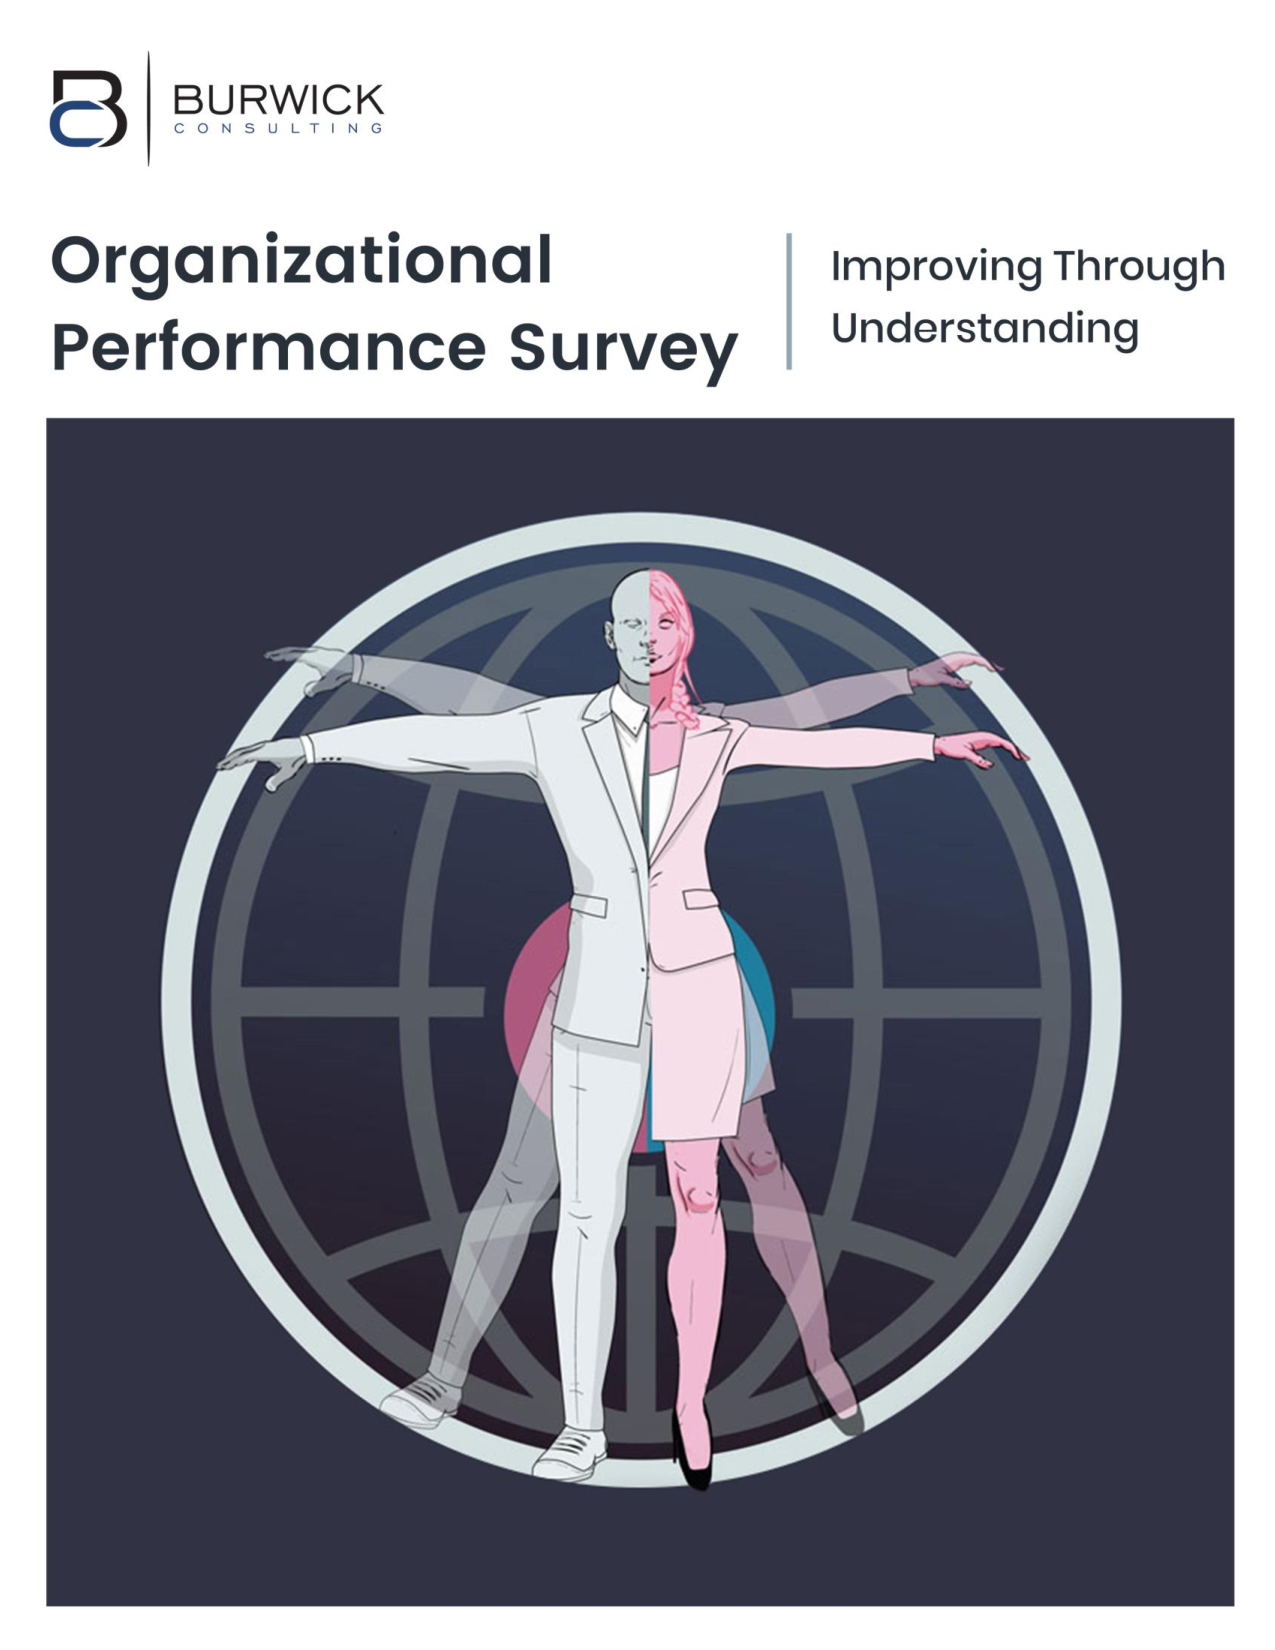
\includepdf[pages={1-}]{SurveyBook}

%\tableofcontents
%^too big

\newpage
\section*{When did you last discuss your performance with your manager?}

\subsection*{\centering Factors Tested}
This question considers management's ability to utilize and create coaching opportunities, develop personnel, deepen relationships, and set goals. Reviewing performance is a meaningful coaching opportunity and the frequency of review matters.
\subsection*{\centering Performance Metrics}
This question has been proven to decrease absenteeism, reduce
safety incidents, improve quality, and improve customer
relationships.
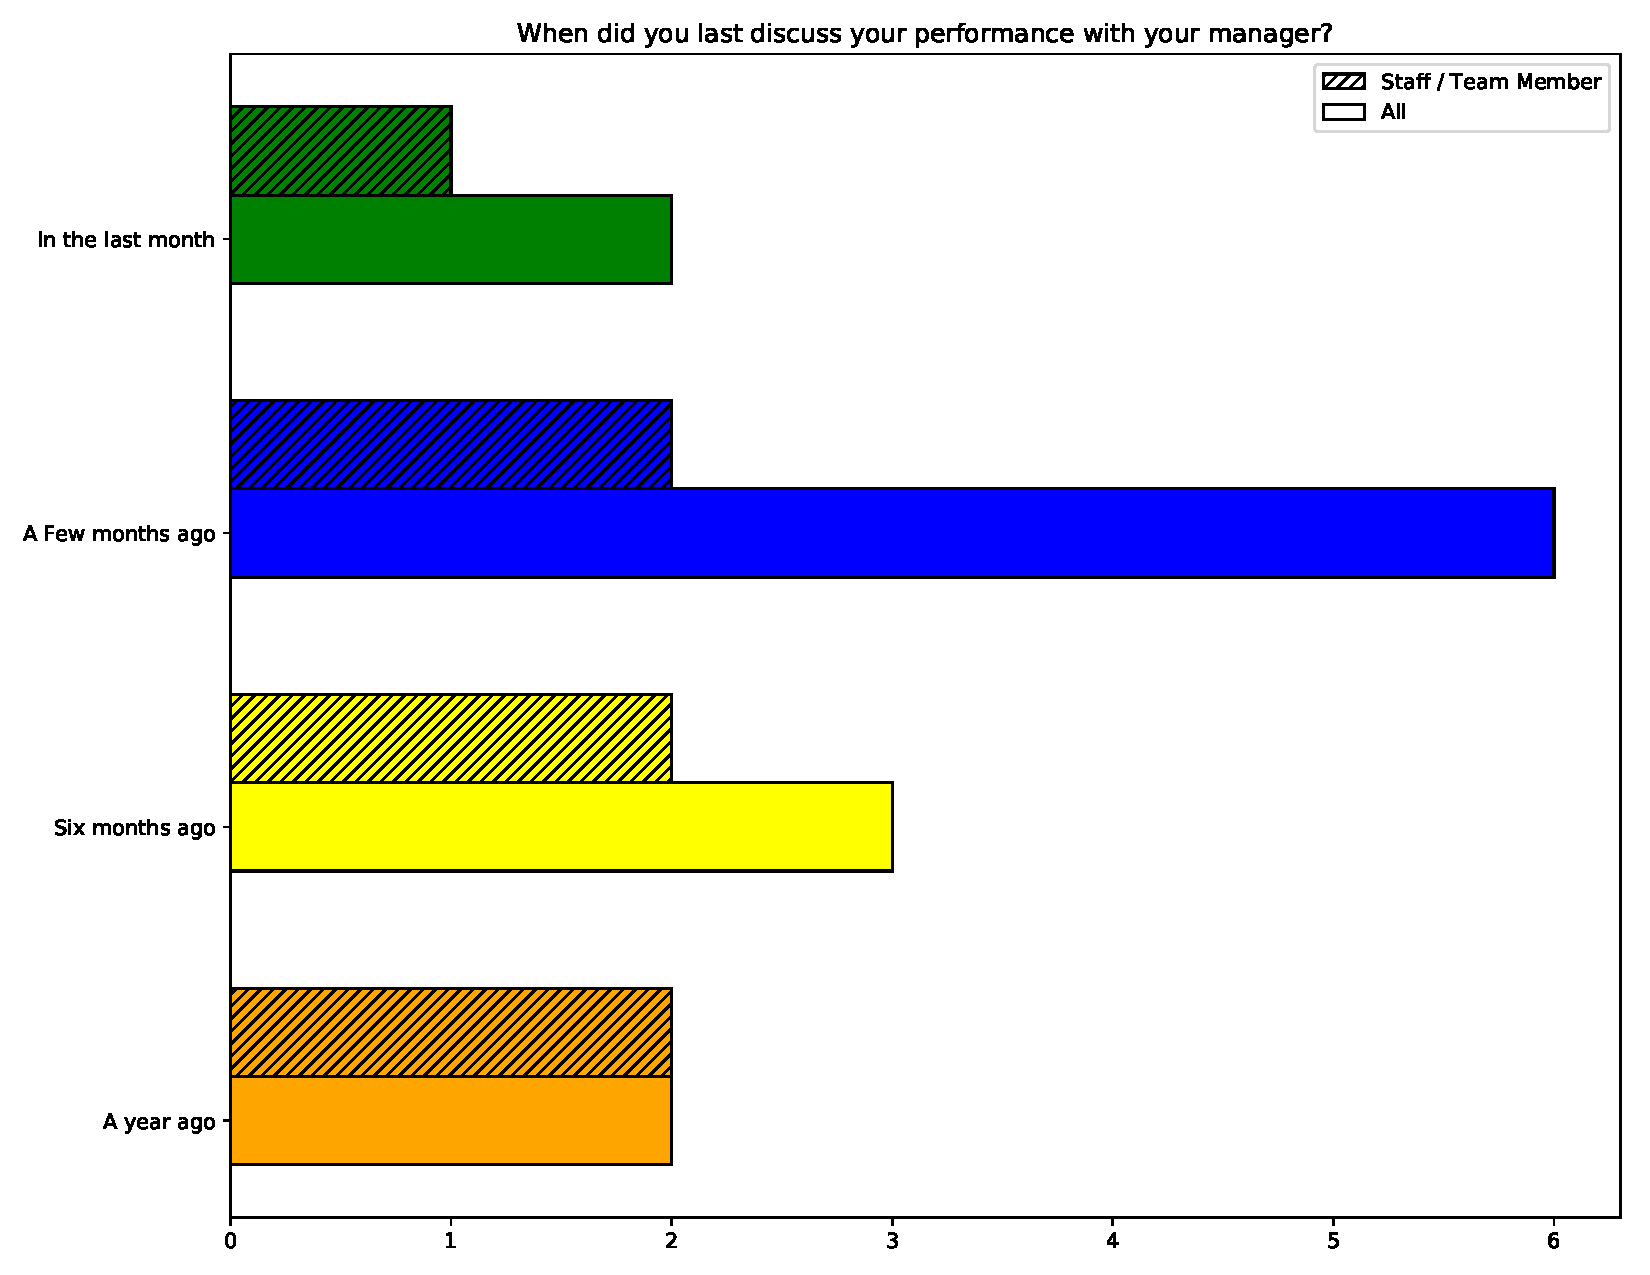
\includepdf[angle=90,origin=c]{q1}
\subsection*{\centering Significance}
84\% of personnel at Company A discuss their performance with a manager more than once a year.
\subsubsection*{}
Recent research into management practices, employee engagement,
behavior and motivation indicate that the annual performance review
may fall short of its objective and should be replaced by coaching and
regular performance reviews.
\subsubsection*{}
Company A is in the top percentage in this category.

\subsection*{\centering Opportunities for Improvement}
To enrich the quality of performance reviews and maximize the time
invested into each employee we suggest that managers use review sessions to set goals for both work performance and discovery of personal goals outside of the office. The same issues people have when completing goals at work likely impact all areas of life. Review sessions are a moment for managers to learn what is meaningful to their people in all aspects of life. This creates stronger teams, motivated employees, and a higher quality of life across the company.

\newpage
\subsection*{\centering Burwick Consulting}
\subsubsection*{}
With over 10 years of coaching and leadership experience, Burwick Consulting trains managers and executives to improve their coaching skills individually or in a group setting.
\subsubsection*{}
Burwick Consulting offers a variety of classes including the science of goals, a tool to help people at any level of an organization learn how to set goals and discover of deep-rooted motivation.

\newpage
\section*{How often do you get to do your best at work?}

\subsection*{\centering Factors Tested}
Creating opportunities for people to do what they do best at work requires management to excel in role design, skills assessments, and personality assessment for job placement. 
\subsection*{\centering Performance Metrics}
The metrics tested by this question have been proven to improve profitability and employee engagement, as well as reducing the number of safety incidents. 
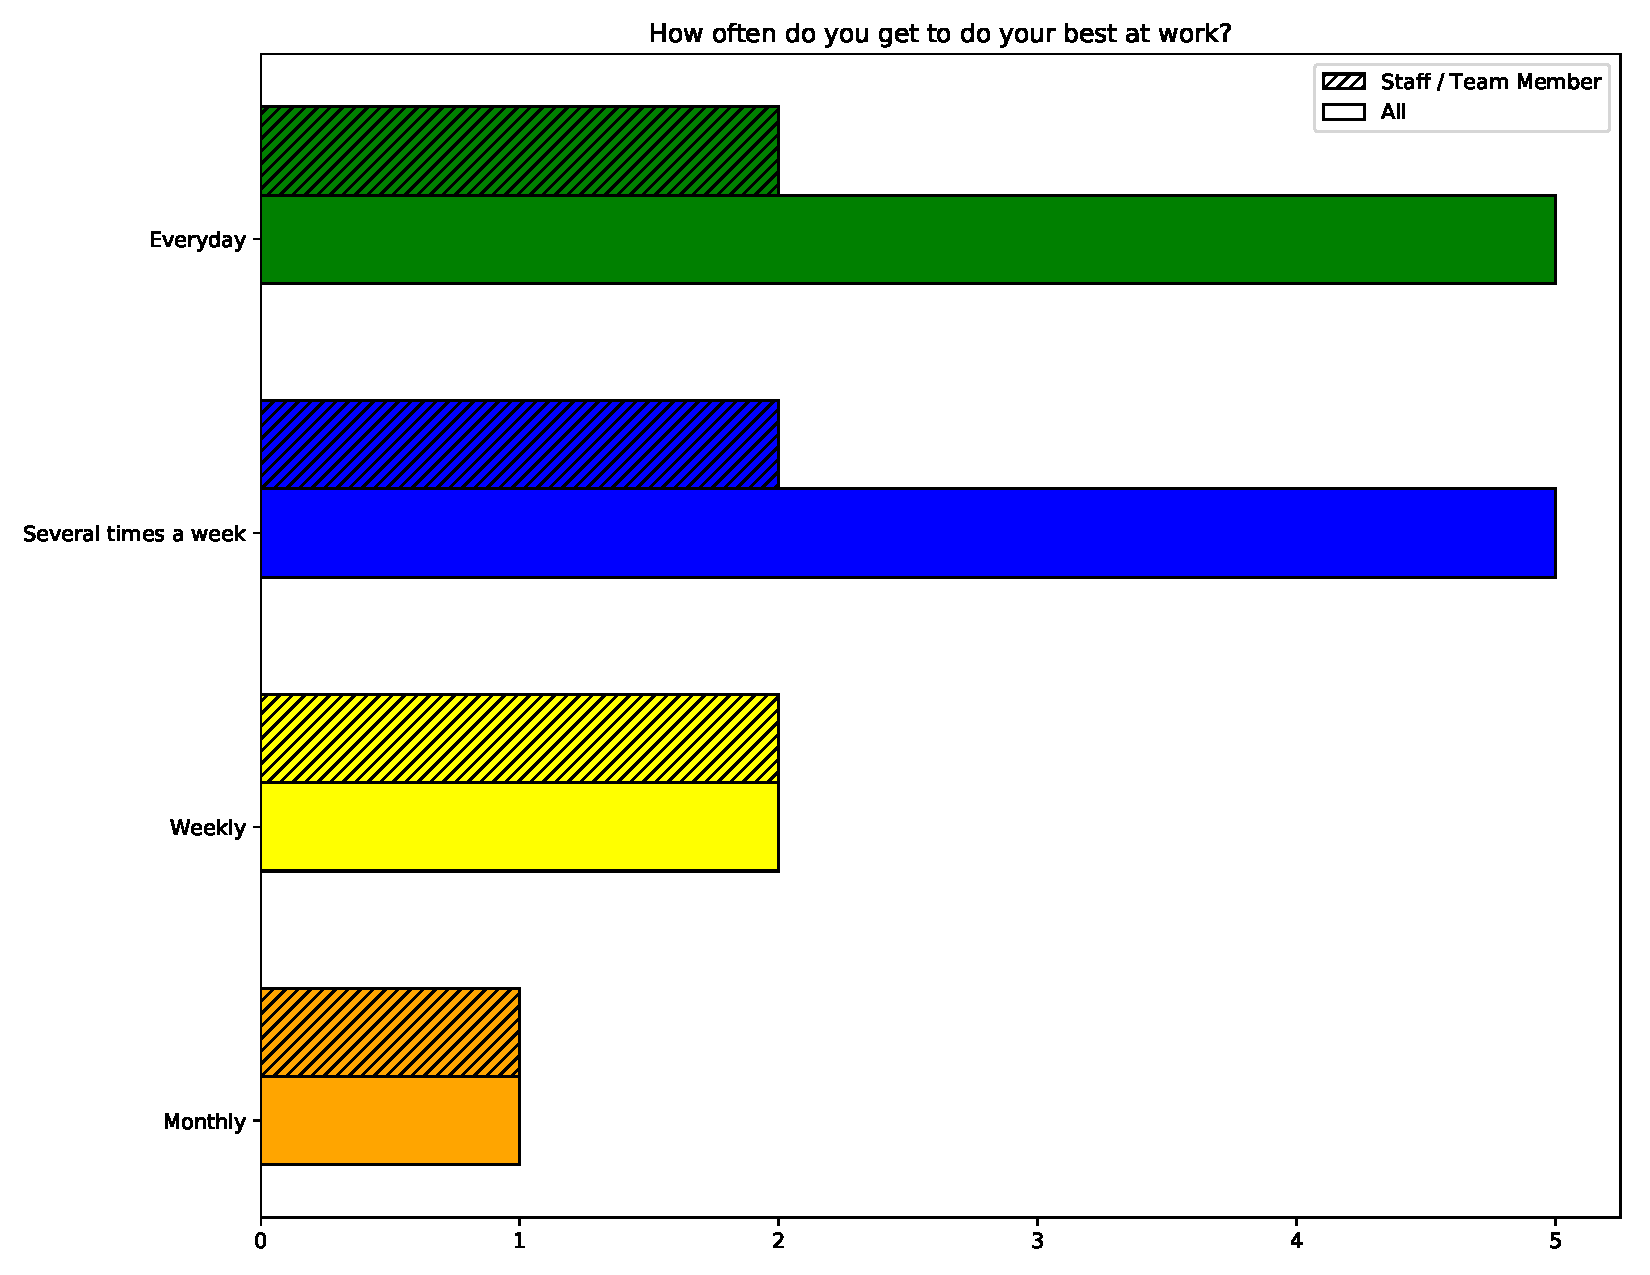
\includepdf[angle=90,origin=c]{q2}
\subsection*{\centering Significance}
38\% of your organization’s personnel report
that they have the opportunity to do what they do best at work everyday.
\subsubsection*{}
Having the opportunity to do what a person does best is a significant
indication of whether a person will find meaning and satisfaction in their work.  This question signifies whether a person's job is psychologically gratifying. According to Gallup, having the opportunity to do what a person does best is the most critical factor when considering whether to take a job at a different organization.

\subsection*{\centering Opportunities for Improvement}
Creating opportunities for personnel to do what they do best at work is complicated. It requires managers to understand the skills and responsibilities of each position. Additionally, it requires that employees possess a degree of self-awareness and can articulate what they are seeking.
\subsubsection*{}
Managers can create an opportunity for employees to do what they do
best at work by focusing on the relationship they have with their
personnel and developing a thorough understanding of each role.
\subsubsection*{}
A great place to learn more about employees is during coaching sessions
while reviewing performance. Managers can work with employees to
identify the employee's skills and strengths and then present the employee with tasks that fit the person.

\subsection*{\centering Burwick Consulting}
Burwick Consulting works with managers and leaders to clarify the tasks and expectations for each position, redevelop roles, and help test an employee’s skills and personalities. 

\newpage
\section*{On a scale of 1-10, 10 being the best score, how comfortable are you sharing new ideas and insights with co-workers?}

\subsection*{\centering Factors Tested}
This question tests the strength of teams as well as management's ability to create an environment of trust and creativity.
\subsection*{\centering Performance Metrics}
The metrics tested by this question have been proven to reduce
turnover and the occurrence of safety incidents while improving
rates of production.
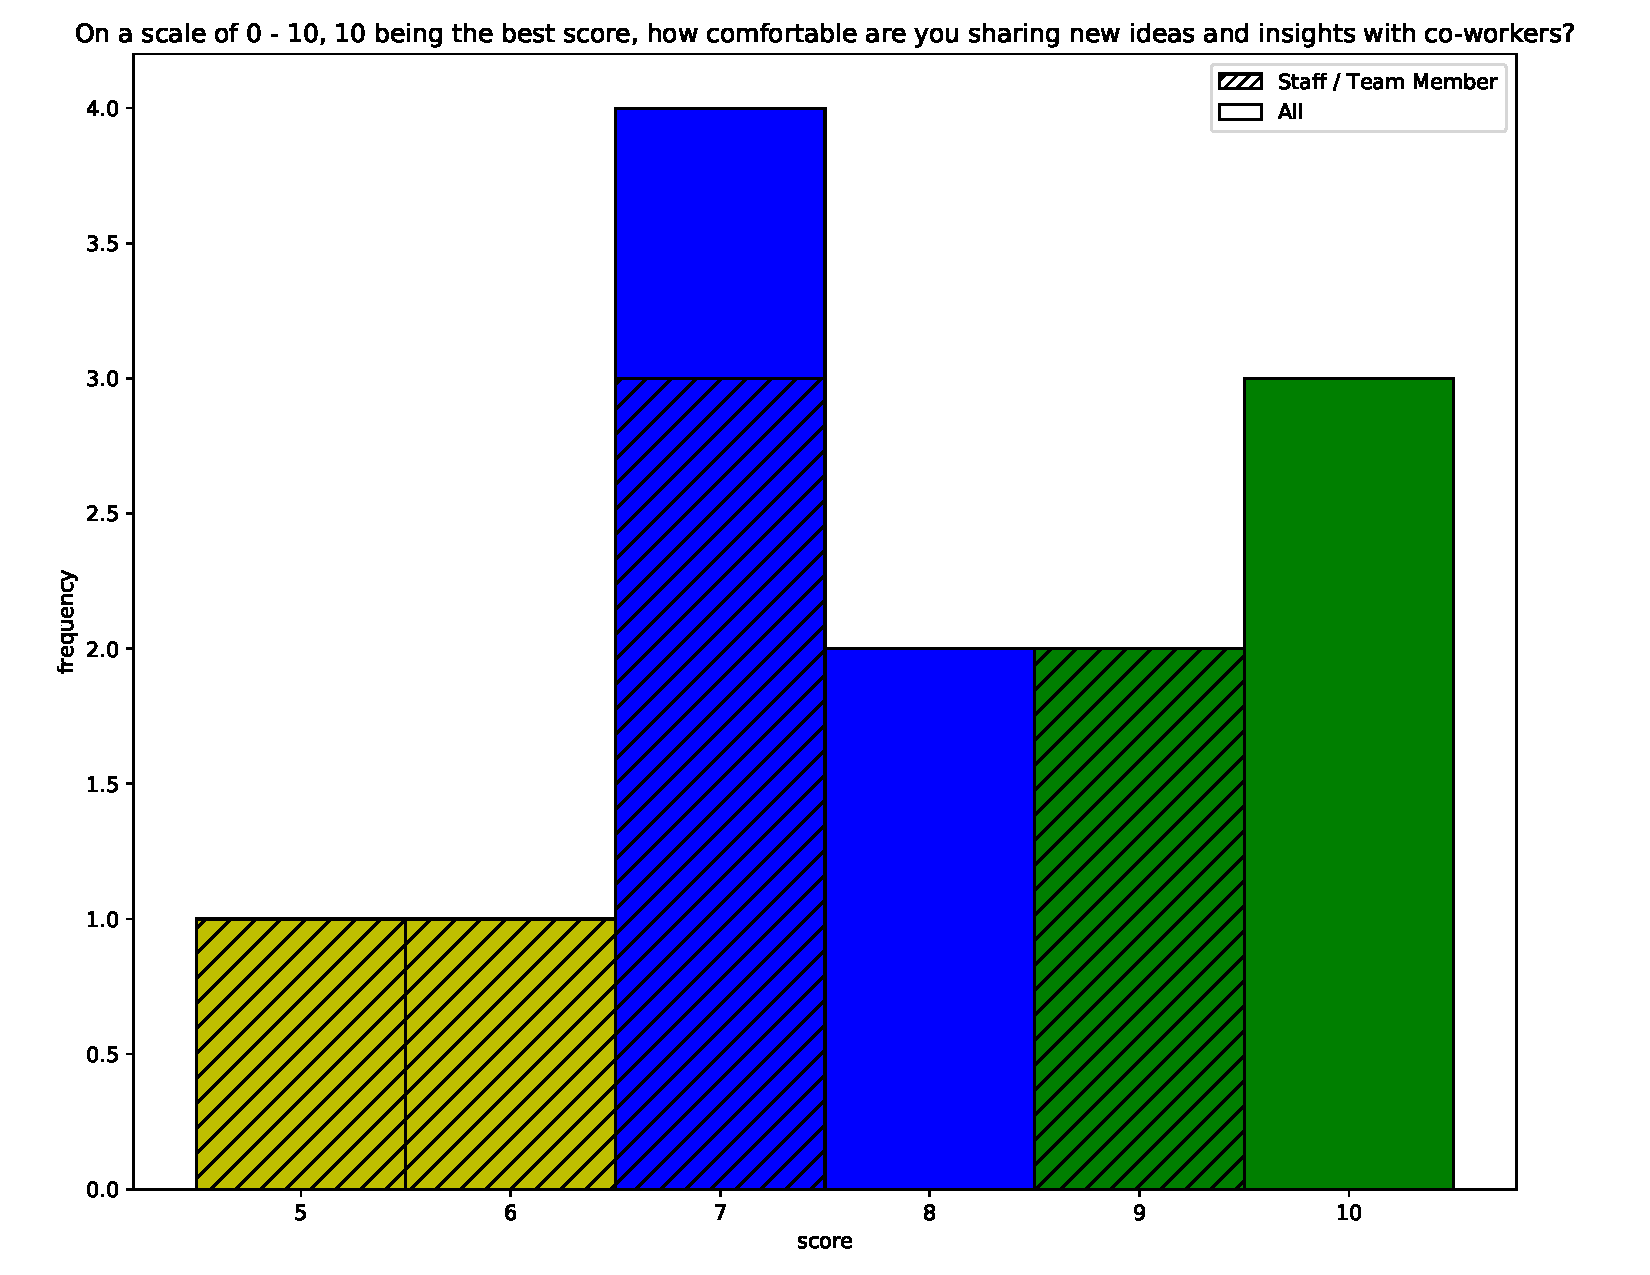
\includepdf[angle=90,origin=c]{q3}
\subsection*{\centering Significance}
53\% of staff and project managers at Company A feel comfortable sharing their ideas most of the time. While 87\%
of Company A’s senior leaders and executives feel comfortable sharing their ideas most of the time.
\subsubsection*{}
The ability to share ideas and insights with co-workers impacts problem
solving and innovation. Although not all ideas are integrated into
solutions, the capacity to see a problem from different perspectives
allows teams to develop creative solutions. When employees don’t feel
comfortable sharing their ideas the whole organization suffers.
\subsection*{\centering Opportunities for Improvement}
To encourage idea sharing among teams, managers can facilitate
discussions. During these conversations, managers should pose a problem and ask for different solutions. Then managers should discuss the benefits of each idea, thereby training their employees to listen for the value of a concept. This type of training encourages team building and a sense of trust.

\subsubsection*{}
Some additional management practices may include: informing employees when their ideas have been integrated into the organization’s strategy; giving feedback on ideas, which may consist of questions to help employees gain clarity on their idea; and creating open calls for solutions to problems that the organization currently faces.

\subsection*{\centering Burwick Consulting}
\subsubsection*{}
Burwick Consulting coaches managers and organizational leaders on how to listen and give encouraging feedback. 
\subsubsection*{}
Additionally, Burwick Consulting facilitates group classes that train teams on how to effectively listen, give feedback, and work through sensitive conversations. 

\newpage
\section*{Do you have the equipment, data, and resources you need to independently do you work?}

\subsection*{\centering Factors Tested}
This question tests management's understanding of the equipment
needed for employees to complete their tasks, whether the
equipment is provided, and the quality of communication.
\subsection*{\centering Performance Metrics}
The metrics tested by this question have been proven to improve
profitability, quality of work and reduce safety incidents.
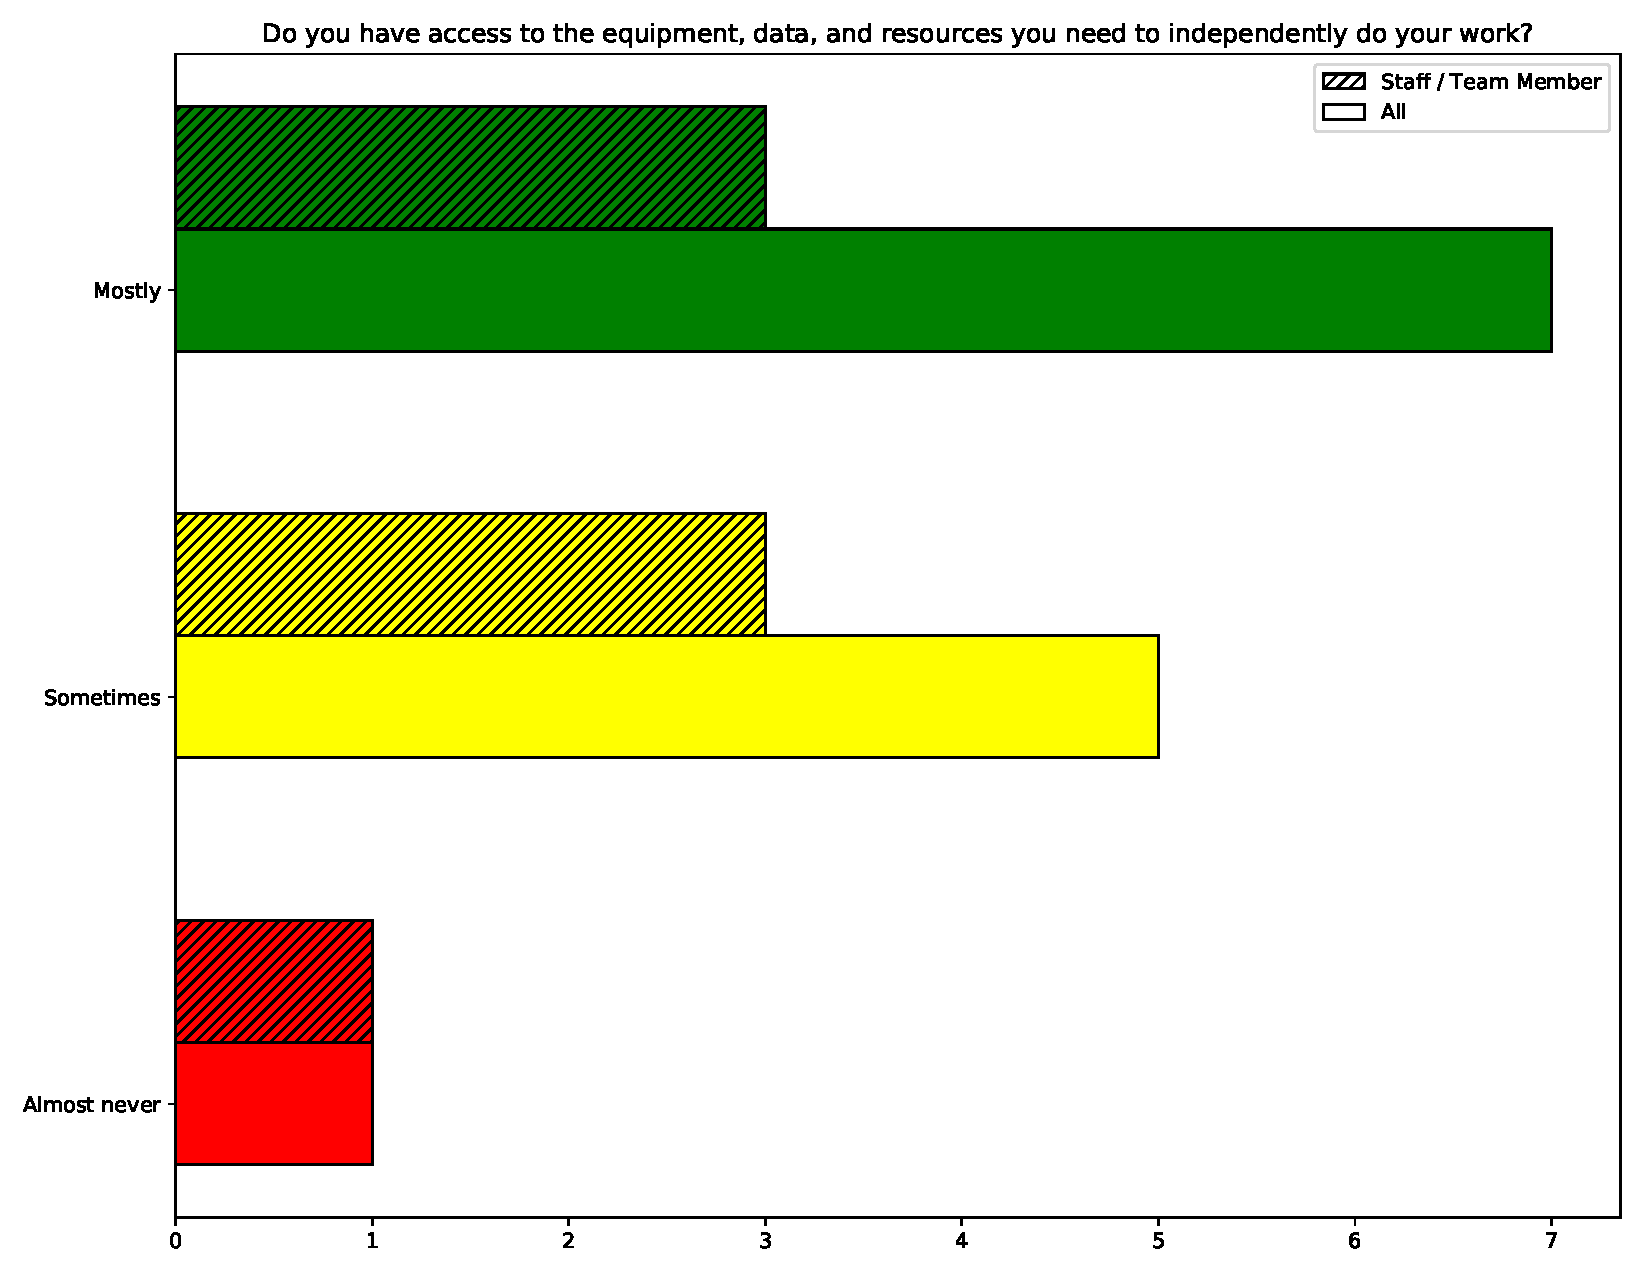
\includepdf[angle=90,origin=c]{q4}
\subsection*{\centering Significance}
46\% of staff members and project managers feel that they do not have all the equipment they need to do their job. While 66\% of senior leaders and executives think that they have the proper equipment to do their job.
\subsubsection*{}
This is significant, according to Gallup, ”having the materials and
equipment to do work well is the strongest indicator of job stress.”

\subsection*{\centering Opportunities for Improvement}
Providing the right tools for every task can be difficult for any organization. Often there are competing interests for finite resources forcing managers to make difficult decisions. When managers share the difficulties they face with their employees, it allows the employees to understand that the lack of supplies is not intentional, which can reduce stress.
\subsubsection*{}
Senior Leaders can also work with employees to identify the essential equipment for job success. 
\subsubsection*{}
Lastly, senior leaders can talk to employees about frustrations with technologies and knowledge gaps to identify other material needs.


\newpage
\section*{Do you feel that you are part of a team working together for a common goal?}

\subsection*{\centering Factors Tested}
This question tests multiple levels of the organization, from
leadership's ability to set goals with clarity, to communicating
those goals to managers and teams, and whether teams are able to
come together to pursue those goals.
\subsection*{\centering Performance Metrics}
The metrics tested by this question have been proven to improve
profitability, cost savings, customer engagement, retention
and reduce absenteeism.
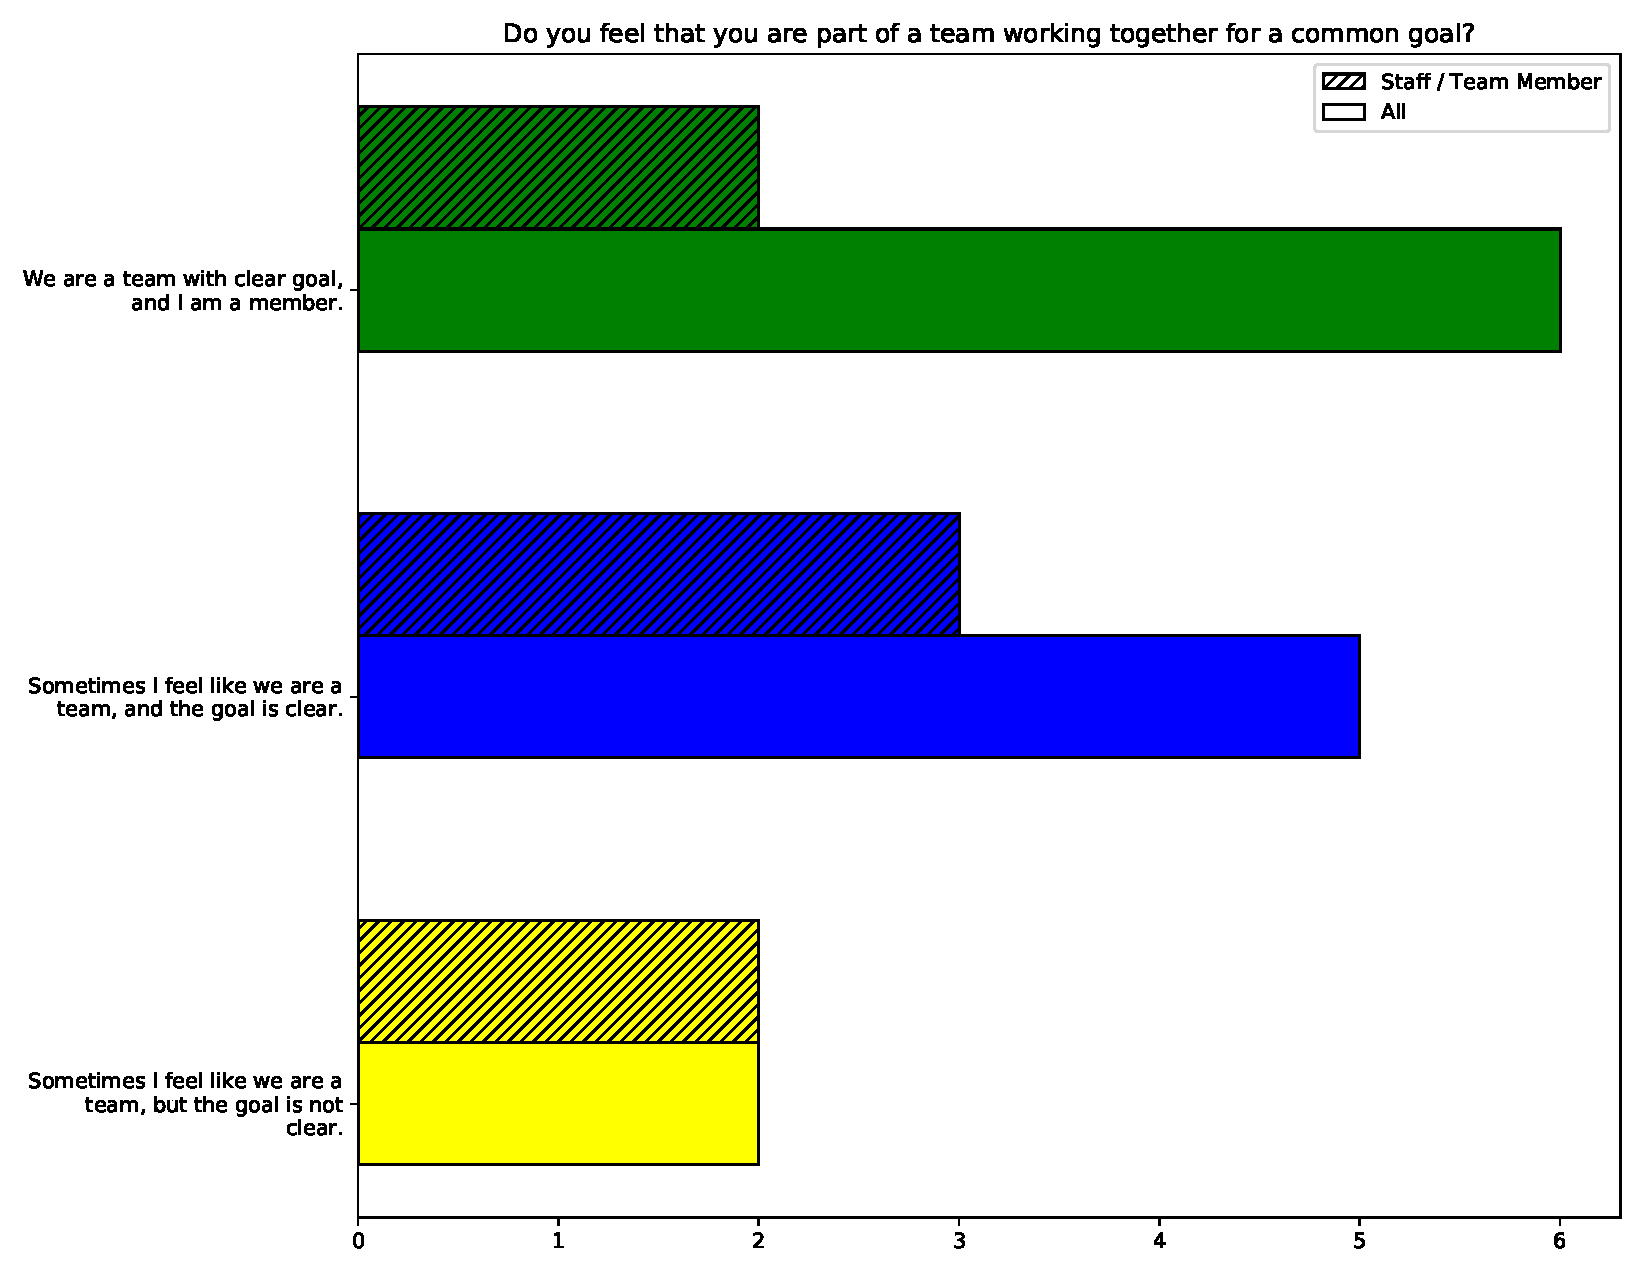
\includepdf[angle=90,origin=c]{q5}
\subsection*{\centering Significance}
This question captures the most comprehensive snapshot of organizational cohesion. For organizations to score well on this question, the entire hierarchy must be operating as a team.
\subsubsection*{}
42\% of all staff members and project managers feel that sometimes we are a
team and the goal is clear.

\subsection*{\centering Opportunities for Improvement}
To create clarity and team cohesion organizational leaders should step back and first clarify, for themselves, the goals of the organization. Next leader and managers can determine whether the goals and strategic objectives are properly reaching the teams. If there is a disconnect between leaders' objectives and the team, managers will need to search for communication breakdowns which can occur for several reasons including lack of reinforcement, issues in clarity, and misalignment of interests.
\subsubsection*{}
Additionally, team cohesion can be enhanced by further inquiring into employee opinions of team dynamics and using the answers as feedback for managers.

\subsection*{\centering Burwick Consulting}
Burwick Consulting works with organizations to understand team dynamics and build strong teams around common goals.

\newpage
\section*{How would you describe your relationships with the people you work with?}

\subsection*{\centering Factors Tested}
This question tests the closeness of the relationships within the
workplace.
\subsection*{\centering Performance Metrics}
Having closer relationships at work, where employees consider
co-workers to be friends has been demonstrated to improve
profitability, productivity, customer engagement, and reduce
safety incidents.
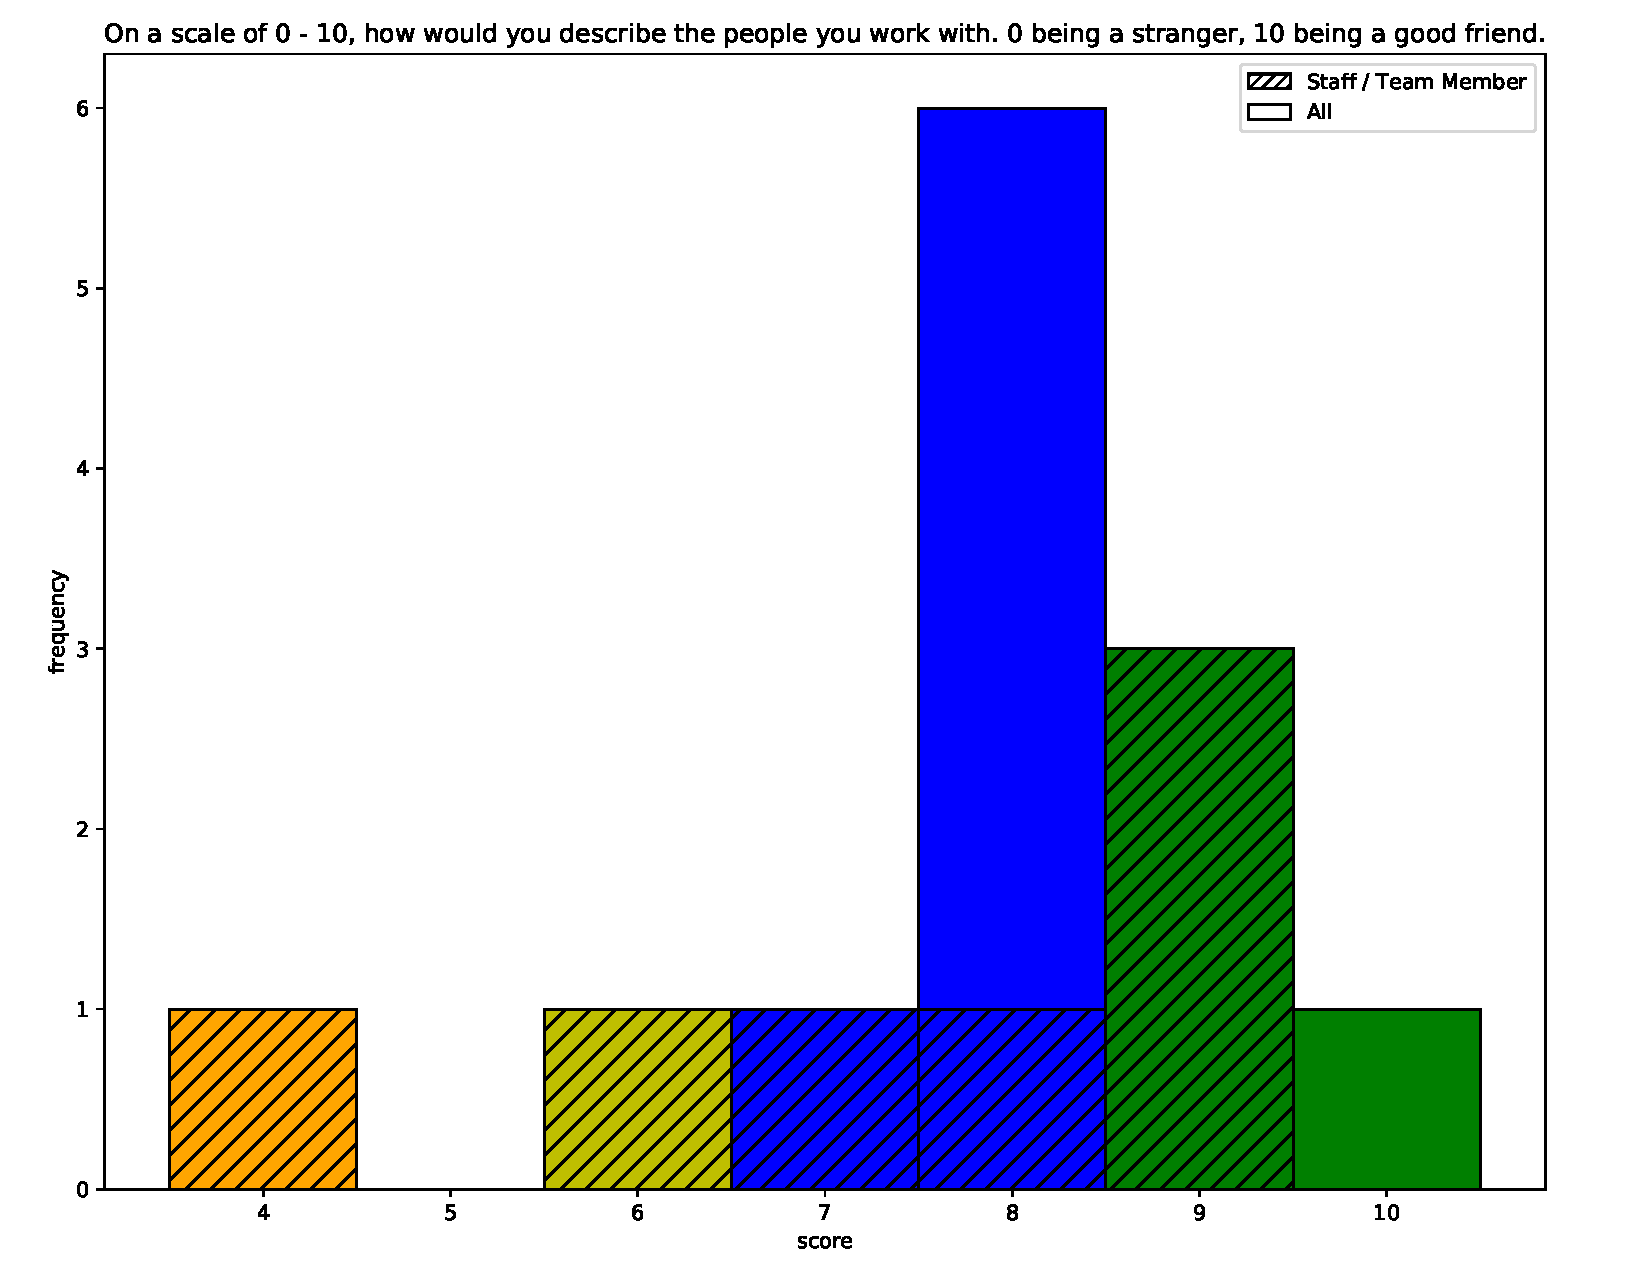
\includepdf[angle=90,origin=c]{q7}
\subsection*{\centering Significance and Opportunities for Improvement}
\subsubsection*{}
"When employees possess a deep affiliation with their team
members, they are driven to take positive actions that benefit the business"
\textit{-Gallup State of the American Workforce}
\subsubsection*{}
It has been a standard convention in the American workforce to
view fellow employees on a strictly professional basis, with a lack
of familiarity. However, the emotional bonds of friendship have
been proven to produce strong effective teams.
\subsubsection*{}
Promoting and cultivating authentic friendships is a difficult task. Improvements in this
metric can be accomplished by shifting leaderships' opinions on
whether employees should be friends and the value those
friendships can bring to the organization.

\newpage
\section*{On a scale of 0 - 10, rate how well your manager knows and supports you with your personal and career goals.}

\subsection*{\centering Factors Tested}
This question tests the authenticity of personal development
from an employee's perspective.
\subsection*{\centering Performance Metrics}
When employees feel that managers are interested in their
success as people, it has been proven that organizations
increase customer engagement and profitability, while reducing
absenteeism and safety incidents.
\newpage
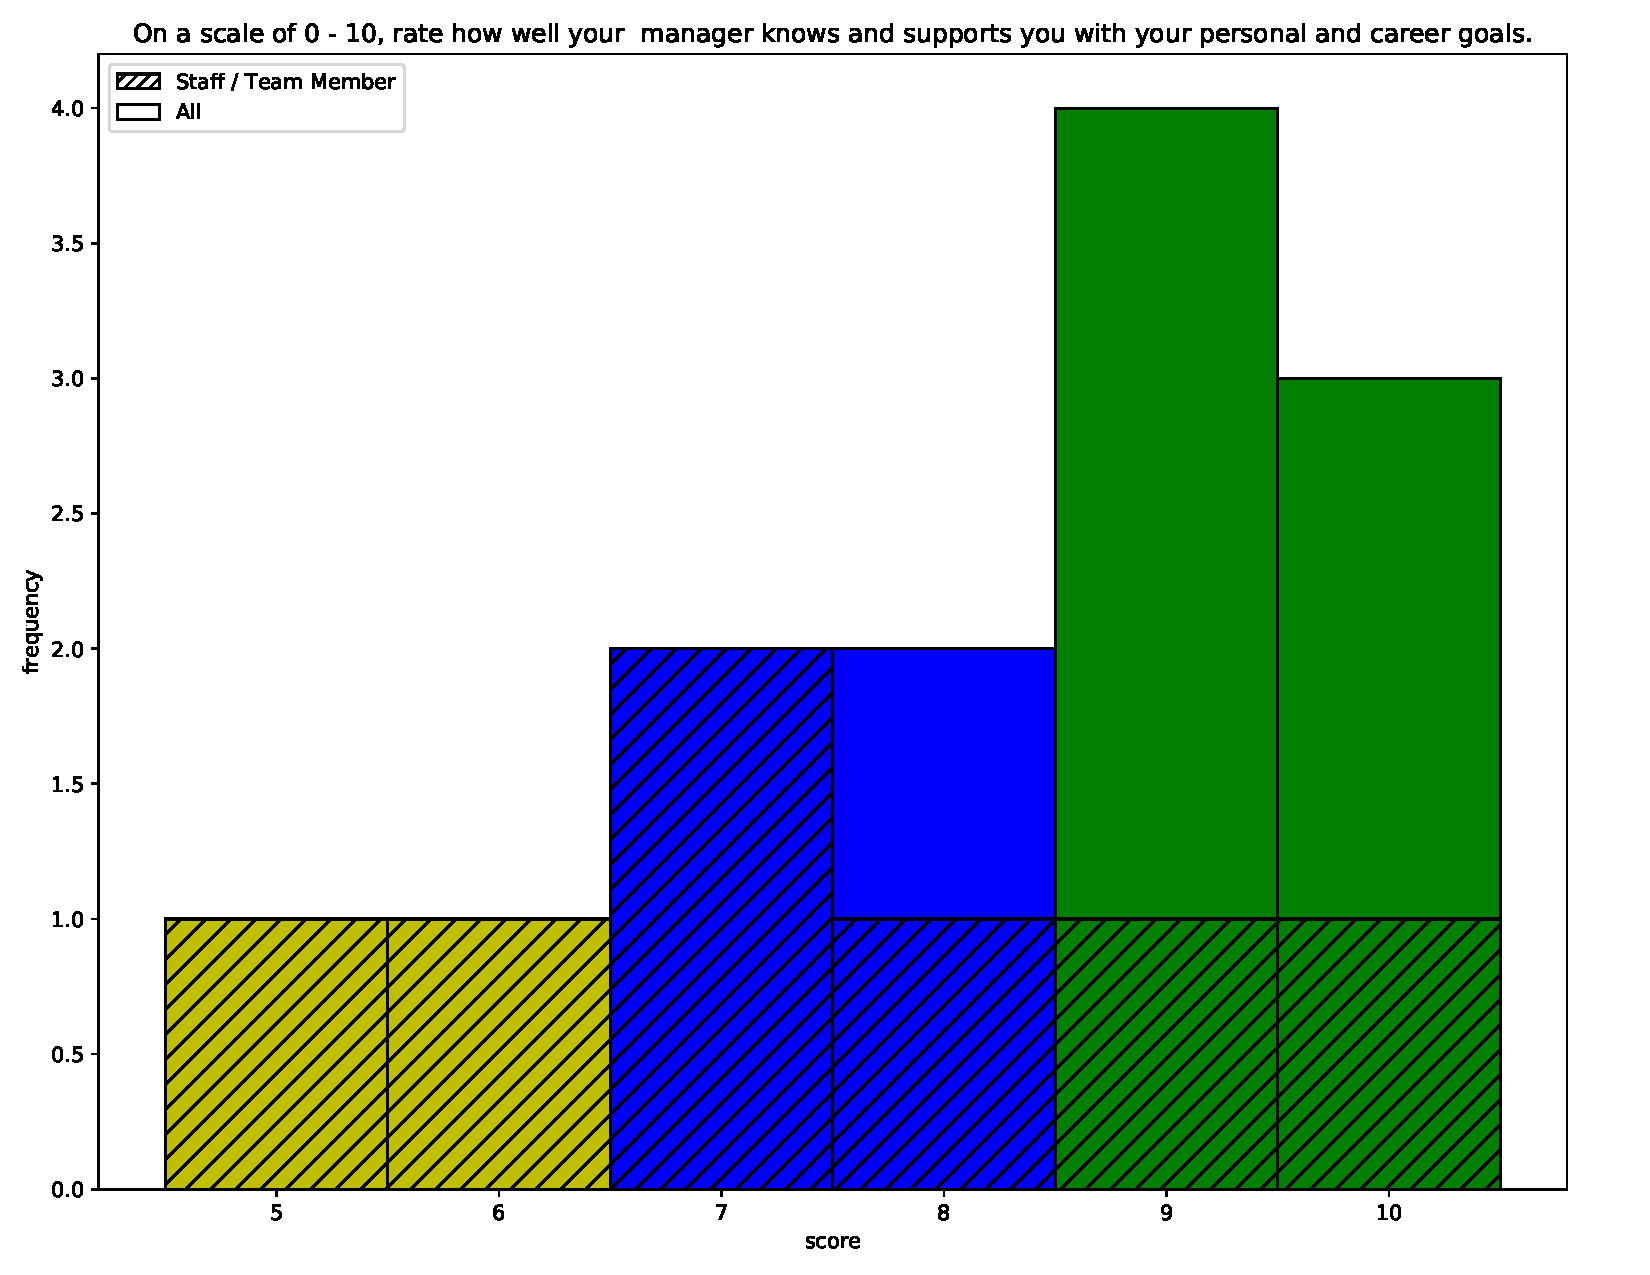
\includepdf[angle=90,origin=c]{q8}
\subsection*{\centering Significance and Opportunities for Improvement}
\subsection*{\centering Factors Tested}
30\% of staff and project managers feel that senior leadership or executives are not interested in their personal or career success. This is a significant number and should raise concerns for both senior leadership and executives.

\subsubsection*{}
The rules for retention in the modern workforce marketplace have changed. Employees are interested in more than just a paycheck and benefits. They want personal and professional development opportunities at work.

\subsubsection*{}
Leaders who know how to effectively coach and bring about the best in their people will be more competitive. When employees feel that their leadership team cares about their success as people, a bond is formed, and employee attitudes shift in a positive direction. Consequently, employees see the office as more than just a workplace; they see it as an extension of who they are and their performance adjusts accordingly.

\subsection*{\centering Performance Metrics}
An excellent method for personalizing feedback and deepening the quality of relationships with employees is learning about their goals that are unrelated to the organization. This should be done during performance review and coaching sessions. Often, performance roadblocks experienced at work stem from the same issues that prevent people from succeeding at home. Consequently learning about and supporting an employee’s goals has two benefits: improved performance at work, and building relationships with employees.


\newpage
\section*{On a scale of 1 - 10, 10 being the highest, how inspiring is your organization's purpose?}

\subsection*{\centering Factors Tested}
Purpose is the articulation of an organization's value proposition
to its clients, it is the organization's reason for being and is
influenced by the vision.
\subsection*{\centering Performance Metrics}
Purpose is the most emotionally significant factor for employees. Purpose impacts long term motivation and has been demonstrated to improve quality
and workplace safety, while strongly reducing absenteeism.
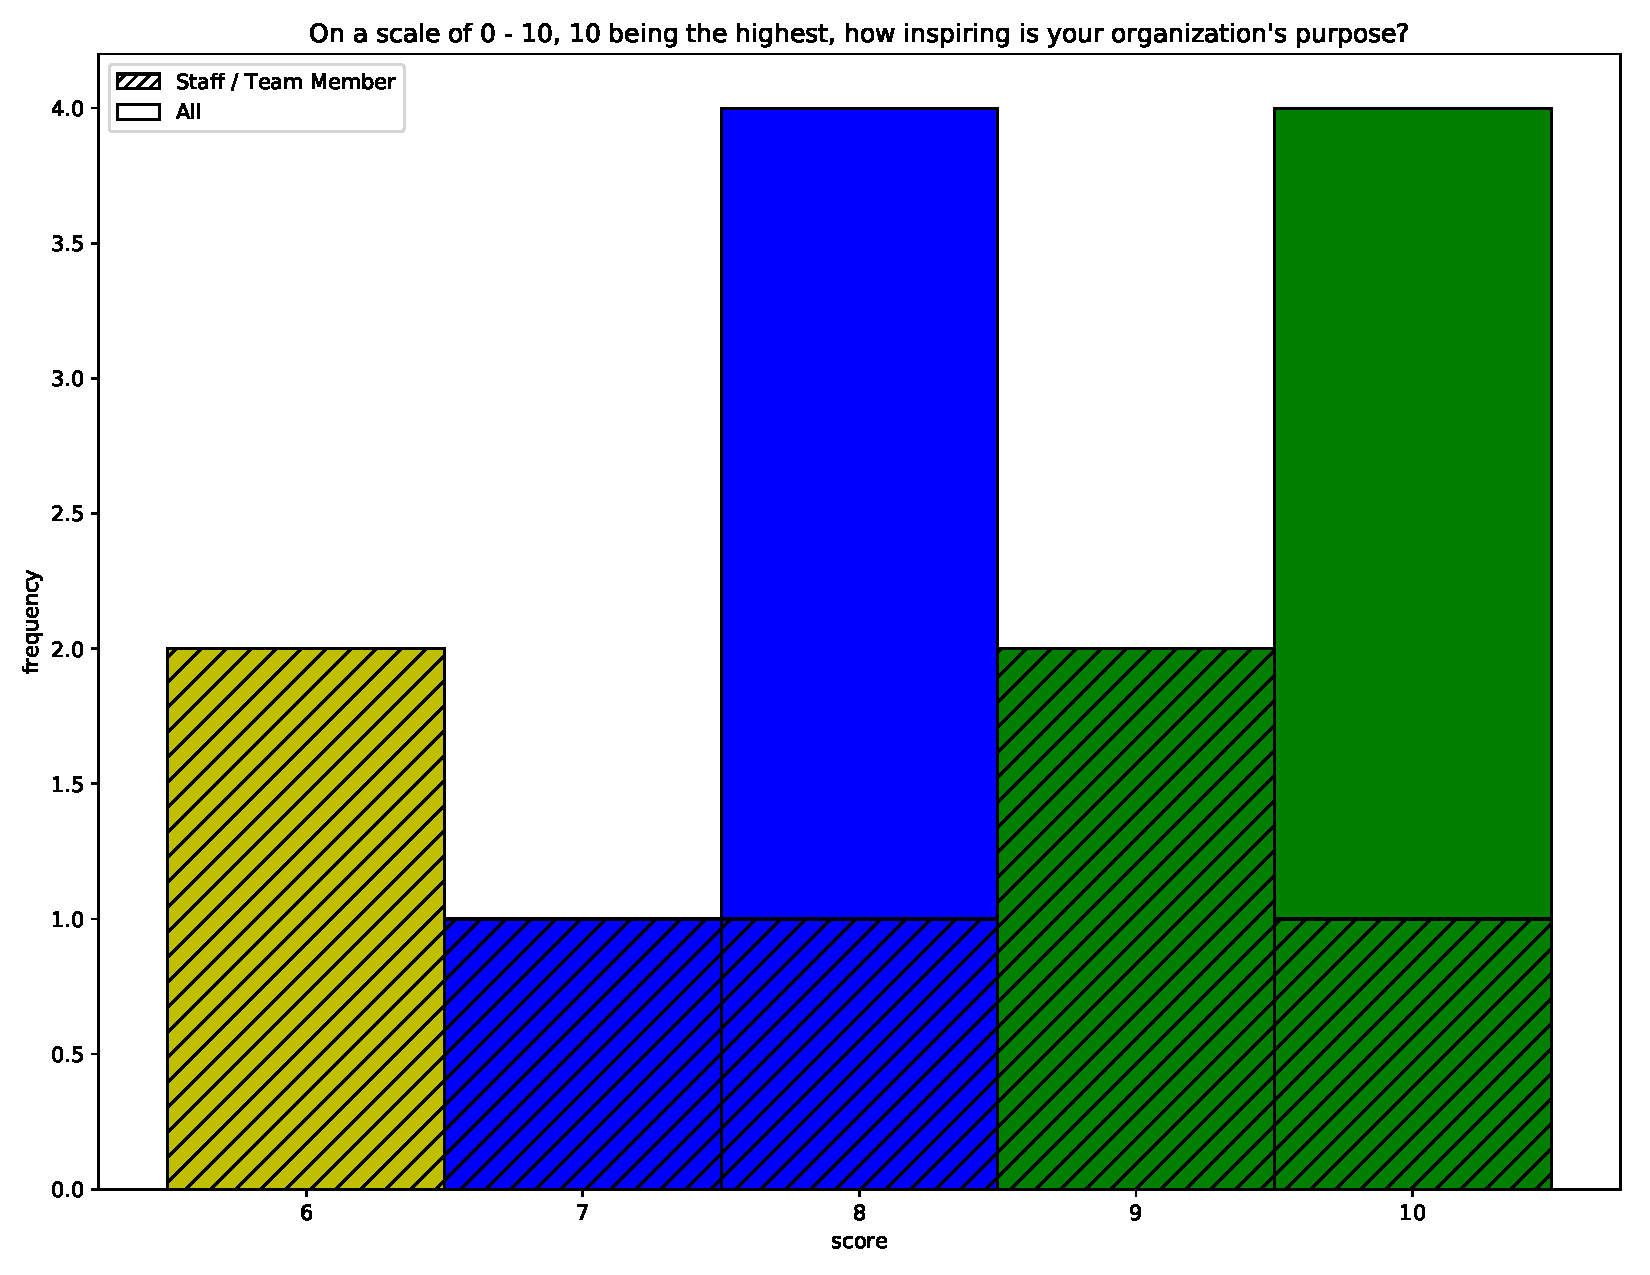
\includepdf[angle=90,origin=c]{q9}
\subsection*{\centering Significance and Opportunities for Improvement}
\subsubsection*{}
This question, in conjunction with the next question, 
tests whether the organization's purpose or mission is
emotionally significant to employees. It also indicates whether
leadership and management are communicating the
organization's purpose in actual communications, strategic
considerations, and actions.
\subsubsection*{}
Defining purpose in an emotionally significant way can be
difficult. To do this, leadership must consider the value they bring
to the people their clients. Value should be thought of as how the
actions of the organization impacts the lives of the people they serve.
\subsection*{\centering Burwick Consulting}
Helps organizational leaders to define actual value, integrate that
into purpose, and align organizational actions with purpose.

\newpage
\section*{What is your organization's purpose? In other words, who are your clients, and how do you help them?}
\begin{center}
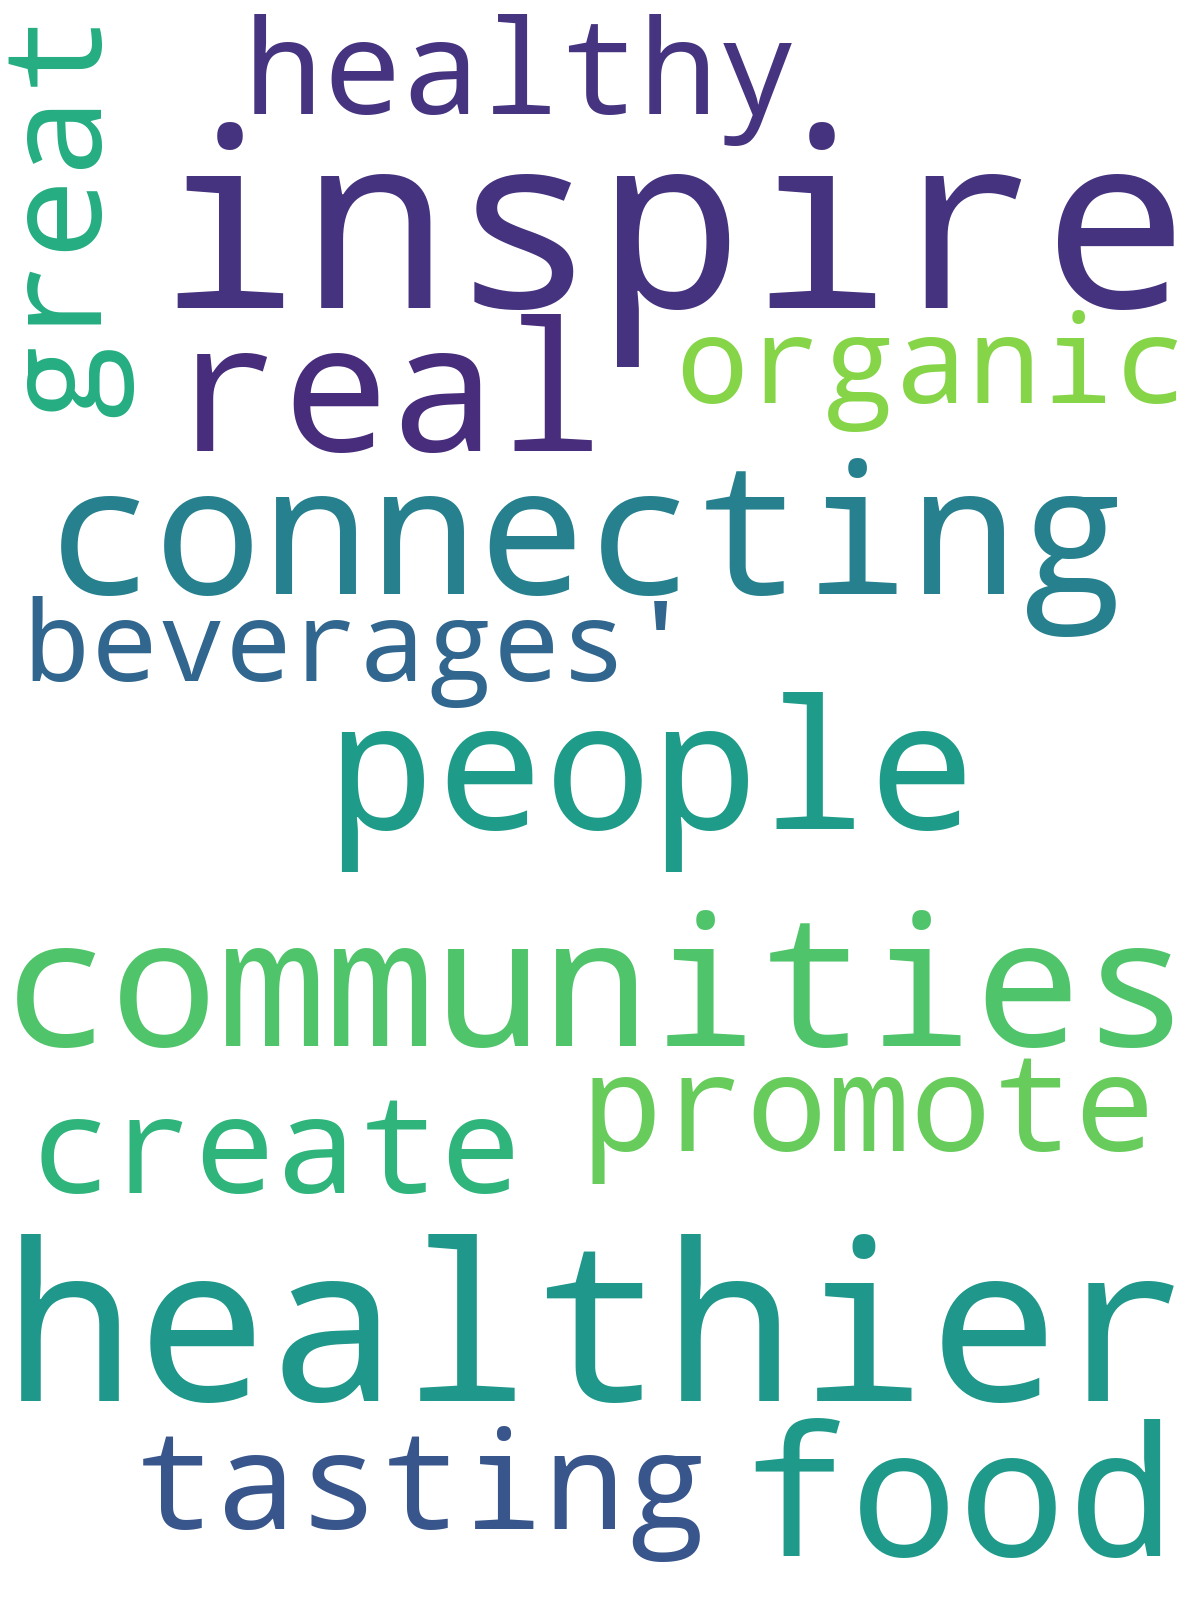
\includegraphics[width=.80\linewidth]{q10}
\end{center}

\newpage
\section*{Tell us your organization's vision}
\subsection*{\centering Factors Tested}
Vision is a critical test for an organization’s leadership. Vision is
more than a collection of words. It is a look into a future that
does not yet exist and is brought to life by the organization.
Vision is the basis of strategy, goal setting, and motivation. This
question not only tests the quality of an organization’s vision, but
also how well the organization communicates that vision through
words and actions to employees on all levels.
\subsection*{\centering Performance Metrics}
Vision is one of the most powerful tools in inspiring employees,
and is a deciding factor when a person is choosing to join a team
or stay with an organization.
\newpage

\includegraphics[width=.95\linewidth]{q11}
\subsection*{\centering Significance and Opportunities for Improvement}
Vision is a powerful tool of strategic alignment and decision
making. Organizational leaders must ask themselves whether the
current strategies align with the vision and often times will need
to adjust if there is any incongruity.
\subsection*{\centering Burwick Consulting}
\subsubsection*{}
Burwick Consulting helps leaders to navigate the difficult task of
strategic alignment and to weigh the considerations that can
stand in the way.
\subsubsection*{}
Additionally, Burwick Consulting helps leaders to structure and articulate
vision in an emotionally compelling way and communicate that
vision throughout the organization.

\newpage
\section*{In a few words, describe your organization's culture}

\subsection*{\centering Factors Tested}
The culture of an organization is a description of the attitudes
and beliefs held by its members. This is an opportunity for
leadership to observe their performance in the eyes of those
they serve.
\newpage
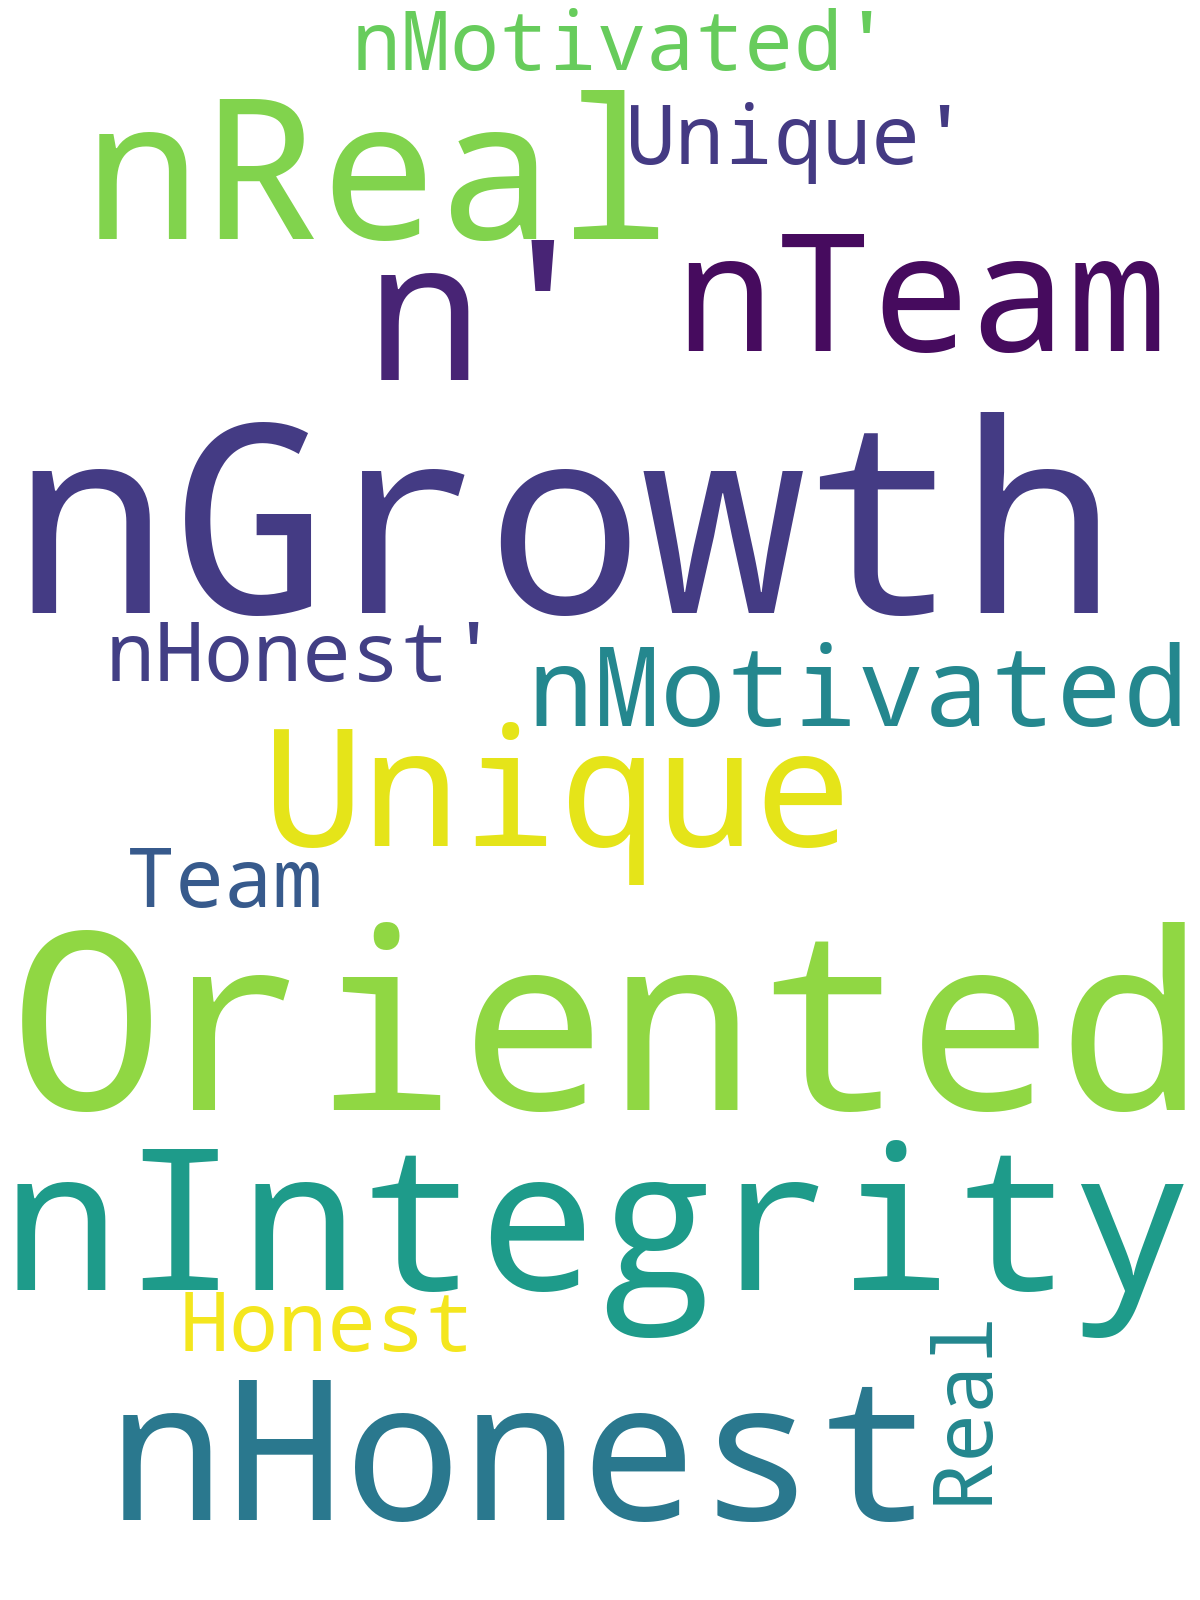
\includegraphics[width=.95\linewidth]{q6}

\newpage

\section*{Bibliography}

\begin{enumerate}
	\item Gartenberg, C., Prat, A. \& Serafeim, G. "Corporate Purpose and Financial Performance.”,
	\item Harvard Business School Working Paper, No. 17-023, September 2016.
	\item Gallup, (2017) State of The American Workplace
	\item Wrzesniewski, A., Schwartz, B., Cong, X., Kane, M., Omar, A. \& Kolditz, T. (2014) “Multiple motives don’t multiply motivation”, Proceedings of the National Academy of Sciences Jul 2014, 111 (30) 10990-10995; DOI:10.1073
	\item Sorich, D. \& Rivera, M (2018) “The Relationship between motivation and owner-operated small business firm business”, Engaged Management Scholarship Conference Temple University.
	\item Woolley, K. \& Fishbach, A. (2016). “For the Fun of It: Harnessing Immediate Rewards to Increase Persistence in Long-Term Goals”, Journal of Consumer Research
	\item Patnaik, D. (2009) “Wired to Care”, Pearson Education
	\item Festinger, L. (1957) “A Theory of Cognitive Dissonance”, Stanford University Press
	\item Doshi, N. \& McGregor L. (2015) “Primed to Perform”, Harper Collins Publishers
	\item Maslow, A (1954) “Motivation and Personality”, Harper and Row
	\item Reik, T (1948) “Listening with the Third Ear”, Noonday Press
	\item Gilovich,T., Griffin, D. \& Kahneman, D. (2002) “Heuristics and Biases”, Cambridge University Press
	\item Perls, F.S. (1969) “Ego, Hunger and Aggression”, Random House New York
	\item Quinn, R. \& Thakor, A., “Creating a Purpose Driven Organization”, Harvard Business Review July - August 2018
	\item Almquist, E., Senior, J. \& Bloch, N., “The Elements of Value”, Harvard Business Review, September 2016
\end{enumerate}

\end{document}